\documentclass[12pt,a4paper,notitlepage]{article}

\usepackage[utf8]{inputenc}

\usepackage[francais]{babel}\usepackage[T1]{fontenc}
\usepackage[cyr]{aeguill}
\usepackage{lmodern}
\usepackage{color}
\usepackage{boites}
\usepackage{fancybox}
\usepackage{listings}
\lstset{language=bash, basicstyle=\footnotesize, frame=shadowbox, rulesepcolor=\color{gris}}


\definecolor{gris}{gray}{0.75}
%\definecolor{bleup}{HTML}{258EE9}


%\renewcommand*\familydefault{\ttdefault} %% Only if the base font of the document is to be typewriter style
%\renewcommand{\rmdefault}{ptm}


\usepackage[
   pdfauthor={Ludovic Terrier & Arnaud Goulut},
   pdftitle={RE12 - TP2},
   ]{hyperref}
   
   
\usepackage[pdftex]{graphicx}

%\usepackage{titlesec}
%\titleformat{\section}[frame] {\normalfont} {\filright
%\footnotesize
%\enspace\textbf{\thesection}\enspace} {8pt} {\Large\bfseries\filcenter}

%% Je contrôle la taille de ma zone imprimée...
\usepackage{anysize}
%% ...en définissants les marges {gauche}{droite}{haute}{basse}
\marginsize{25mm}{15mm}{10mm}{15mm}

\begin{document}

\title{La configuration réseau sous Linux (2)}
\author{Arnaud Goulut et Ludovic Terrier}
\date{Avril 2010}
\maketitle


%\tableofcontents

\thispagestyle{empty}


%%%%%%%%%%%%%%%%%%%%%%%%%%%%%%%%%%%  1ère page 


%%%%%%%%%%%%%%%%%%%%%%%%%%%%%%%%%%% 1ère partie
\section{Partie 1 : Les niveaux d'exécution}

\subsection{Paramétrage du service réseau}
On retrouve le paramétrage du service réseau dans le fichier : \texttt{/etc/init.d/network} :

\begin{lstlisting}
#! /bin/bash
#
# network       Bring up/down networking
#
# chkconfig: 2345 10 90
# description: Activates/Deactivates all network interfaces configured to \
#              start at boot time.
#
### BEGIN INIT INFO
# Provides: $network
# Should-Start: iptables ip6tables
### END INIT INFO
\end{lstlisting}

La ligne contenant chkconfig nous indique que ce service est par défaut démarré dans les runlevels 2, 3, 4 et 5 avec la priorité 10. De plus, il est stoppé dans les autres runlevels (1 et 6) avec la priorité 90. 

\subsection{Exécution des scripts}

Les commandes liées à l'exécution des scripts sont situées dans le dossier \texttt{/etc/init.d/} qui sont les cibles des liens symboliques situées dans le dossier \texttt{/etc/rcX.d}, où \texttt{X} est le numéro du runlevel.


\subsection{La commande chkconfig}
Cette commande permet de modifier le paramétrage des différents services dont celui du réseau. On peut tout d'abord vérifier les états au démarrage d'un service donné pour chaques runlevels avec la commande :

\begin{lstlisting}
chkconfig --list network
\end{lstlisting}
De plus, on peut modifier l'état au démarrage d'un service pour les runlevels avec la commande :
\begin{lstlisting}
chkconfig --level 5 network off
\end{lstlisting}
Dans ce cas, le service \texttt{network} ne démarrera pas dans le runlevel 5.


\section{Partie 2 : le super-serveur xinetd}
\subsection{Configuration de telnetd}
 
Dans le cadre du TP la configuration de telnetd pour xinetd a simplement consisté en l'installation de ces deux paquets. En effet, en installant telnet sur une machine xinetd s'installe automatiquement. De plus, l'installation créée automatiquement le fichier de configuration du service telnet pour xinetd dans le répertoire \texttt{/etc/xinet.d/telnet}. Dans ce fichier il faudra cependant mettre \texttt{no} à la place de \texttt{yes} à la ligne suivante :
\begin{lstlisting}
       disable		= no
\end{lstlisting}

\subsection{Les services à rattacher à xinetd}
Il est préférable de rattacher à xinetd des services qui sont peu utilisés, tels des services d'accès à distance. En revanche, pour des services recevant de nombreuses connections (tel que web, ldap et messagerie) on n'utilisera pas xinetd.

\subsection{Capture de session telnet}
\begin{figure}[!h]
\begin{center}
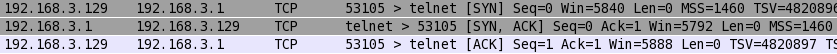
\includegraphics[height=1cm]{syn_ack.png}
\caption{Etablissement d'une connexion TCP pour telnet.}
\label{fig:do}
\end{center}
\end{figure}

Nous voyons ici les échange SYN, SYN/ACK et ACK à l'initiative du client pour établir la connexion telnet. Nous pouvons remarquer le port utilisé par le client : 53105.  Le Maximum Segment Size (MSS) est de 1460 octets et la fenêtre (Win) à une taille de 5840 octets pour le client.

\begin{figure}[!h]
\begin{center}
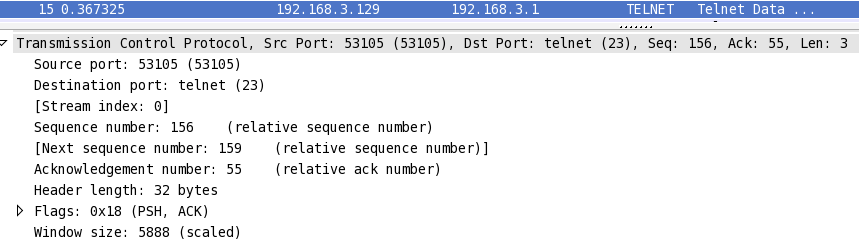
\includegraphics[height=4cm]{pck15.png}
\caption{Paquet numéro 15 de la communication TCP.}
\label{fig:do}
\end{center}
\end{figure}

La figure précédente montre en détail le contenu TCP du paquet 15. Le client envoie l'Ack 55, c'est à dire qu'il attend l'octet 55 dans le prochain paquet. On remarque aussi la taille de la fenêtre (\og Windows size\fg) que est de 5888 octets. Dans le paquet suivant on voit qui le serveur envoie quant-à lui le paquet numéro 55 (Seq). Ce qui correspond bien aux attentes du client.

\begin{figure}[!h]
\begin{center}
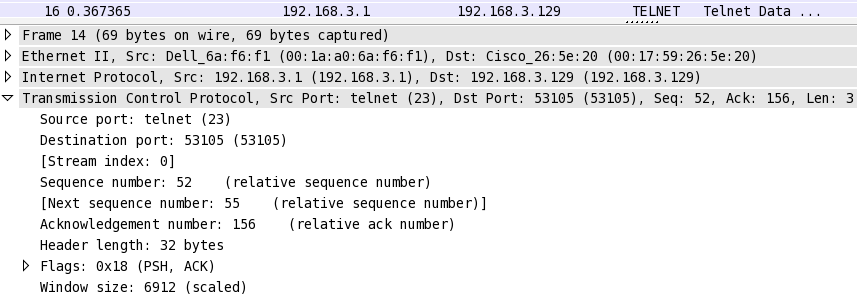
\includegraphics[height=4cm]{pck16.png}
\caption{Paquet numéro 16 de la communication TCP.}
\label{fig:do}
\end{center}
\end{figure}

\subsection{Filtrage d'accès}

Il existe deux moyens pour filtrer l'accès à un service : 
\begin{itemize}
\item via les fichiers \texttt{/etc/hosts.allow} et \texttt{/etc/hosts.deny} (utilisant le TCP Wrapper),
\item dans le fichier de configuration du service.
\end{itemize}

\subsubsection{\texttt{host.deny} et \texttt{host.allow}}

\noindent Pré-requis : le fichier allow est prioritaire sur le fichier deny.\\

\begin{lstlisting}
# /etc/hosts.deny: list of hosts that are _not_ allowed to access the system.
ALL EXCEPT in.telnetd: 192.168.3.0/255.255.255.0
\end{lstlisting}
Ainsi, avec la ligne suivante on autorise personne (\texttt{ALL}) sauf pour le service telnet (\texttt{in.telnetd}) qui sera autorisé pour le réseau local (\texttt{192.168.3.0}).


\subsubsection{fichier de configuration}

\begin{lstlisting}
# default: on
service in.telnetd
{
       flags		= REUSE
       socket_type	= stream
       wait		= no
       user		= root
       server		= /usr/sbin/in.telnetd
       only_from	= 192.168.3.0
       log_on_failure	+= USERID
       disable		= no
}
\end{lstlisting}

\subsubsection{permissif ou restrictif?}



La stratégie qui semble la plus sûre est celle utilisant un filtrage restrictif puisque l'on spécifie explicitement ce que l'on veut autoriser; donnant plus de contrôle sur les accès à destination de la machine.


\section{Partie 3 : Serveurs d'accès distant}

\subsection{Attache à xinetd}

Pour rattacher un nouveau service à xinetd, il suffit de créer un fichier de configuration dans \texttt{/etc/xinet.d/} en ajoutant le paramètre \texttt{server\_args = -i} et en stoppant le service ssh: \\

\begin{lstlisting}
# default: on
service ssh
{
       flags		= REUSE
       socket_type	= stream
       wait		= no
       user		= root
       server		= /usr/sbin/sshd
       server_args	= -i
       log_on_failure	+= USERID
       disable		= no
}
\end{lstlisting}

Après divers tests on s'aperçoit que le temps d'accès au service ssh n'est que sensiblement augmenté après le rattachement de celui-ci à xinetd.





\end{document}